\documentclass[11pt,a4paper]{article}
\usepackage{pdfpages}
\usepackage{helvet}
\usepackage{graphicx}
\usepackage{color}
\usepackage{pgf}
\usepackage{rotating}
\usepackage{eurosym}
\usepackage{wrapfig}
\usepackage{setspace}
\usepackage{eso-pic}
\usepackage{subfig}
\usepackage{afterpage}
\usepackage{sidecap}
%\usepackage[numbers]{natbib}
\usepackage{enumitem}
%\usepackage{natbib}
\usepackage{aas_macros}
%\usepackage{url}
\usepackage{hyperref}
\usepackage{multirow}
\usepackage[percent]{overpic}
\usepackage{booktabs}
\usepackage{latexsym}
\usepackage{pdfpages}

\textwidth=18 truecm
\textheight=26.6 truecm
\voffset=-3.4 truecm
\hoffset= -2.5 truecm % was 0.5

\setcounter{tocdepth}{1}

\def\lsim{\raise0.3ex\hbox{$<$\kern-0.75em\raise-1.1ex\hbox{$\sim$}}}
\def\gsim{\raise0.3ex\hbox{$>$\kern-0.75em\raise-1.1ex\hbox{$\sim$}}}

\newcommand{\muK}{\mu  {\rm K}} 
\newcommand{\muKarcmin}{\mu  {\rm K\cdot  arcmin}}
\newcommand{\kmbysbyMpc}{\,{\rm km~s^{-1}~Mpc^{-1}}}
\newcommand{\comred}[1]{\textcolor{red}{#1}}
\newcommand{\comblue}[1]{\textcolor{blue}{#1}}

%====================================================================================
\usepackage{amssymb,amsbsy,amsmath,amsfonts,amssymb,amscd}
\usepackage{setspace}
\newcommand{\FIX}[1]{\textbf{$\blacktriangleleft$ #1 $\blacktriangleright$}}


%====================================================================================
%Mission names
\newcommand{\core}{\textit{\negthinspace CORE}}
\newcommand{\coreplus}{\textit{\negthinspace COrE+\/}}
\newcommand{\corepp}{\textit{\negthinspace COrE++\/}}
\newcommand{\Planck}{\textit{\negthinspace Planck\/}} \newcommand{\planck}{\textit{\negthinspace Planck\/}}
\newcommand{\Spitzer}{\negthinspace \textit{Spitzer\/}}
\newcommand{\Herschel}{\textit{\negthinspace Herschel\/}}
\newcommand{\prism}{\textit{\negthinspace PRISM\/}}
\newcommand{\Euclid}{\negthinspace \textit{Euclid\/}}
\newcommand{\WMAP}{\negthinspace \textit{WMAP\/}}
\newcommand{\SPICA}{\negthinspace \textit{SPICA\/}}
\newcommand{\SOFIA}{\negthinspace \textit{SOFIA\/}}

%====================================================================================
\newcommand{\ME}{\,M\euro}
\def\m{\ifmmode $m$\else \,m\fi}

\newcommand{\dg}{\nobreak^\circ}
\newcommand\NB[1]{\noindent\underline{N.B.{#1}}~: }
\newcommand{\eg}{\textit{ e.g. }}
\newcommand{\ie}{\textit{ i.e.\ }}
\newcommand{\cf}{\textit{ cf.}}
\newcommand{\etal}{\textit{ et~al.\ }}
\newcommand\etc{\textit{ etc.}}
\newcommand{\rms}{\emph{ rms } }
\def\st{\ifmmode ^{\mathrm{st}} \else $^{\mathrm{st}}$\fi}
\def\nd{\ifmmode ^{\mathrm{nd}} \else $^{\mathrm{nd}}$\fi}
\def\rd{\ifmmode ^{\mathrm{rd}} \else $^{\mathrm{rd}}$\fi}
\def\th{\ifmmode ^{\mathrm{th}} \else $^{\mathrm{th}}$\fi}

\newcommand\ltsima{$\; \buildrel < \over \sim \;$}
\newcommand\simlt{\lower.5ex\hbox{\ltsima}}
\newcommand\gtsima{$\; \buildrel > \over \sim \;$}
\newcommand\simgt{\lower.5ex\hbox{\gtsima}}
\newcommand\simprop{\lower.5ex\hbox{$\; \buildrel \propto \over \sim \;$}}
\newcommand\mypar[1]{\smallskip\par\noindent\textbf{#1}}
\newcommand{\Msolar}{M_\odot}
\newcommand{\jim}[1]{\textcolor{red}{\bf #1}}
\newcommand{\fixme}[1]{\textcolor{red}{#1}}

%====================================================================================


\newcommand{\note}[1]{}
% To see notes uncomment this version:
%\newcommand{\note}[1]{{\color{red} #1}


\begin{document}
\section{Telescope}
In this section, the choice of telescope design will be considered. The optical performance of two configurations will be examined, a Gregorian design and a cross-Dragone design. These two designs will now be examined, highlighting the advantages and disadvantages of each, as applicable to the \coreplus mission, whose requirements are high polarization purity, 6~arcminute resolution at 145~GHz, mirrors less than 1.5$\times$1.6~m, minimising weight and a large focal plane to accommodate several thousand detectors from 60-600~GHz. \comblue{Darragh: That sentence is a bit of a placeholder. The figures I took for resolution and detector numbers come from last year's proposal submitted to ESA} In each case a primary mirror of effective diameter 1.2~m was assumed, satisfying the science requirements.

\subsection{Gregorian Design}
The Gregorian design, with unoptimised reflector surfaces, is an off-axis dual reflector telescope with a parabolic primary reflector and an ellipsoidal secondary \cite{granet_2002}. This mission calls for a large diffraction limited field of view (DLFOV) over the frequency range 60-600~GHz. Considering this, and the limitations imposed by the volume available in which to house the telescope and associated optics and focal plane architecture, various Gregorian configurations were examined. Figure \ref{fig:gregschem} shows a particular design that was considered in some detail. 
\begin{figure}[htbp]
	\centering
	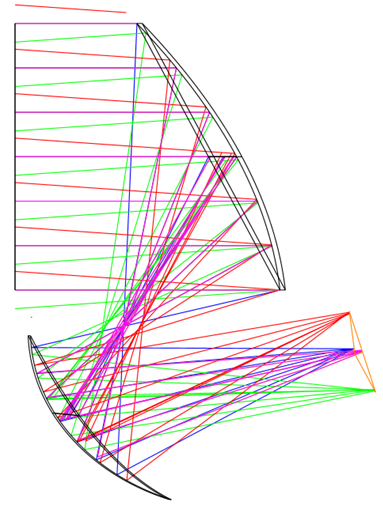
\includegraphics[scale=0.5]{core_greg_nolens.png}
	\caption{1.2~m Gregorian design}
	\label{fig:gregschem}
\end{figure}
In order to realise optimal performance, the mirrors were optimised using aspheric surfaces. The primary mirror has dimensions 1.36~m $\times$ 1.20~m (length $\times$ width), and the secondary mirror is 0.97~m $\times$ 0.67~m. These mirrors fit within the mechanical limits which allow them to be manufactured as one section, which has significant benefit in terms of cost and mechanical complexity.

This design has an 8~deg field of view and realises a usable focal plane that is approximately 40~cm in diameter (with F/\#1.6 at the centre) at 60~GHz, which is determined by examining the Strehl ratio on the focal plane. 0.8 is taken to be the value below which the system is no longer diffraction limited, so plotting this contour reveals the diffraction limited focal plane available at a given frequency. 

The focal plane provides a usable detector area across the band, however in order to achieve this it was necessary to use a curved focal plane surface, which is a limitation of this design. The advantages and disadvantages of Gregorian designs, in the context of this mission, are shown below. \comblue{Darragh: I tried to save some space by cutting out the Strehl ratio plot of the design that we only really use as a lead in to the lens design. I will put the Strehls for the lens design later in the doc. I am not sure taking it out is the best idea, but is it okay if we're pushing to save space?}


\textbf{Advantages:}
\begin{itemize}
	\item Compact design
	\item Reflectors are small, compared to other telescope configurations
	\item Easier to effectively baffle for stray light than other telescope configurations
	\item Focal plane is located close to the base of the payload module. This is advantageous in terms of cryogenic and mechanical complexity
\end{itemize}

\textbf{Disadvantages:}
\begin{itemize}
	\item Gregorian design has inherently smaller focal plane than other telescope types
	\item Focal plane surface is not flat, which is complex for planar coupling schemes
	\item Although easier to effectively baffle, the required baffling configuration is demanding and is a tight fit within the available volume
\end{itemize}
The most significant disadvantage outlined above is that of the focal plane shape. This would not pose such a large problem if horns were an option for the detector technology. As described earlier, with approximately 3000 detectors required, horn arrays are mechanically heavy and difficult to cool. Therefore, arrays of lens-coupled  Kinetic Inductance Detectors (KIDs) are proposed. These must be carefully aligned according to the profile and depth of the focal plane in order to be normal to the incoming beams and to avoid defocussing effects. Owing to the dimensions of the wafers on which the KIDs are manufactured, it is not possible to satisfactorily achieve this on such a curved focal plane. If the Gregorian is to be used, it is therefore necessary to use additional tertiary optics to obtain a flat focal plane architecture.

In order to investigate this, a design with primary and secondary mirrors of dimensions 1.50~m $\times$ 1.30~m and 1.00~m $\times$ 0.70~m was used. An alumina lens was also included between the secondary mirror and the focal plane as a way to flatten the focal plane, as shown in figure \ref{fig:gregschem_lens}. 
\begin{figure}[htbp]
	\centering
	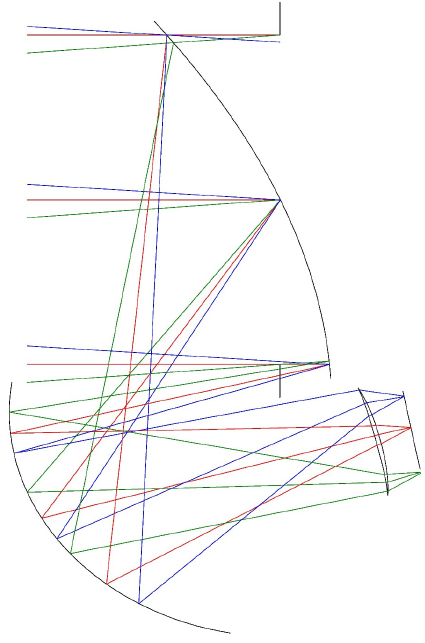
\includegraphics[scale=0.5]{core_greg_lens.png}
	\caption{1.2~m Gregorian design with alumina lens}
	\label{fig:gregschem_lens}
\end{figure}

\begin{figure}[htbp]
	\centering
	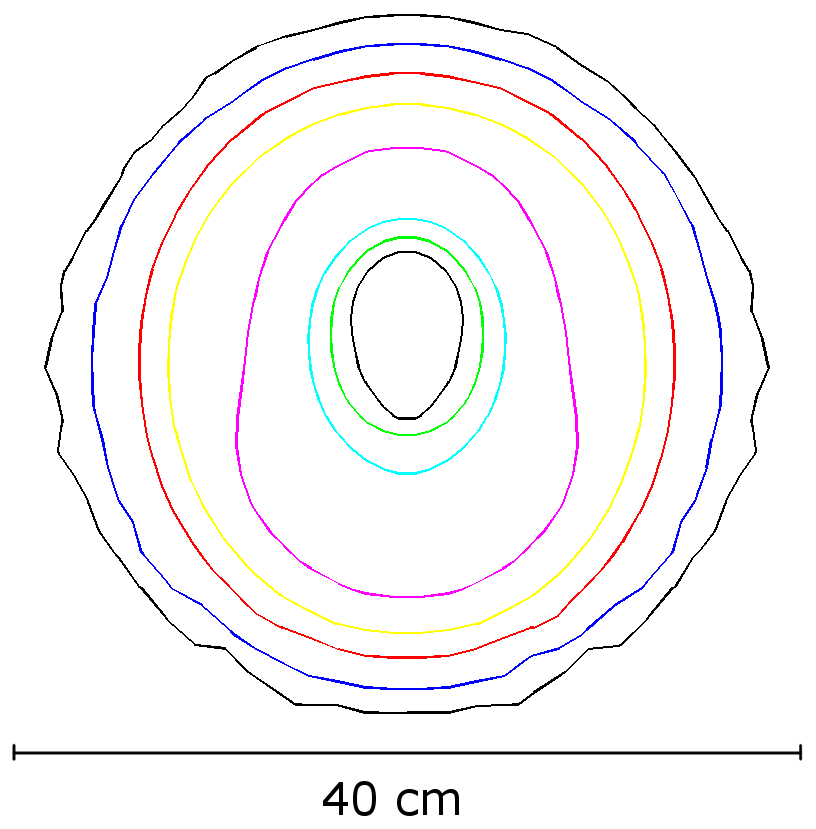
\includegraphics[scale=0.5]{core_greg_lens_strehl.png}
	\caption{Contours where Strehl ratio $= 0.8$ for 60~GHz (black, outer), 90~GHz (blue), 130~GHz (red),
                 160~GHz (yellow), 220~GHz (magenta), 340~GHz (cyan), 450~GHz (green), and 600~GHz (black, inner).
                 }
	\label{fig:greg_lens_strehl}
\end{figure}
This design provides an approximately 8~deg field of view. The lens is 44~cm in diameter (optically it is 42~cm in diameter, but a mounting flange of 1~cm is required), and is estimated to have a mass of approximately 6~kg. The diffraction limited focal plane is 1.1~m, and so a focal plane unit with a diameter of approximately 40~cm can now be realised, including the effects of the lens. The contours representing the DLFOV for various frequencies across the band are shown in figure \ref{fig:greg_lens_strehl}. It can be clearly seen in figure \ref{fig:gregschem_lens} that the focal plane surface is now flat, and so the issue regarding the placement of the focal plane pixels has been resolved. Although the lens addresses the main issue of the Gregorian with the non-telecentric focal plane, it presents a number of additional complications. The most significant of these is the potential for the lens to introduce significant instrumental wavelength dependent polarization effects, in addition to the necessity for a broadband anti-reflection coating.

As a flat focal plane is a firm requirement that is driven by the detector technology that is to be used, a cross-Dragone design is now examined as this provides a naturally flat focal plane without the need for tertiary optics.

\subsection{Crossed Dragone}

The Crossed Dragone configuration \cite{tran_2008, granet_2001} naturally has a large 
field of view and a flat, telecentric focal plane making it a promising CMB telescope design. 

%reasons for crossed dragone

The \coreplus optical design is a modified Crossed Dragone using mirrors defined by an anamorphic aspheric 
surface rather than conic sections. 
The anamorphic asphere is a surface with different radii of curvature in $x$ and $y$, $z$ is parallel to 
the chief ray, 
%\comred{(our coordinates aren't really Az-El anymore since the system has been rotated on it's side.)} 
as well as higher order deformation terms.
The CodeV definition is 
%\begin{equation}
$$ z = \frac{\frac{x^2}{R_x^2} + \frac{y^2}{R_y^2}}
{ 1 + \sqrt{1 - (1+k_x) \frac{x^2}{R_x^2} - (1+k_y) \frac{y^2}{R_y^2}}}
+ A_{n,r} ( (1-A_{n,p})x^2 + (1 + A_{n,p})y^2)^n
% + B_r ( (1-B_p)x^2 + (1 + B_p)y^2)^3 + . . . 
$$
%\end{equation}
where $R_x$ and $R_y$ are the radii of curvature, $k_x$ and $k_y$ are the conic coefficients, and $A_{n,r}$, $A_{n,p}$
define the higher order deformation of the surface. In our design $2 \leq n \leq 5$. When the higher order terms are zero this 
type of surface is often referred to as a biconic.

The basis of our system came from the LiteBIRD telescope design, a 40~cm crossed dragone using anamorphic 
aspheres 
\cite{litebird} \comred{what do we cite for this? Karl will ask Tomo, who gave us the files}, which we scaled up to 1.2~m. 
This base design has a long focal length, f/2.5, to allow 
for baffling the focal plane.  After scaling to a 1.2~m aperture the mirror shapes and offsets were optimized 
in CodeV to maximize the DLFOV \comblue{Darragh: I updated my section to define the abbreviation in the introduction} for the full \coreplus bandwidth, 60-600~GHz.  
Figure \ref{fig:raytrace_xdragone} 
shows the raytrace of this design. The f/\# was appoximately maintained, with a final value of f/2.54 at the 
center of the focal plane.
The focal plane is flat and telecentric with a DLFOV greater than 10 degrees across at 150 GHz, significantly larger than the 
Gregorian case.  DLFOV as deffined by Strehl $=0.8$ contours are shown in Figure~\ref{fig:strehl_xdragone}.


%ray trace with/without fold?
\begin{figure}[htbp] %  figure placement: here, top, bottom, or page
	\centering
	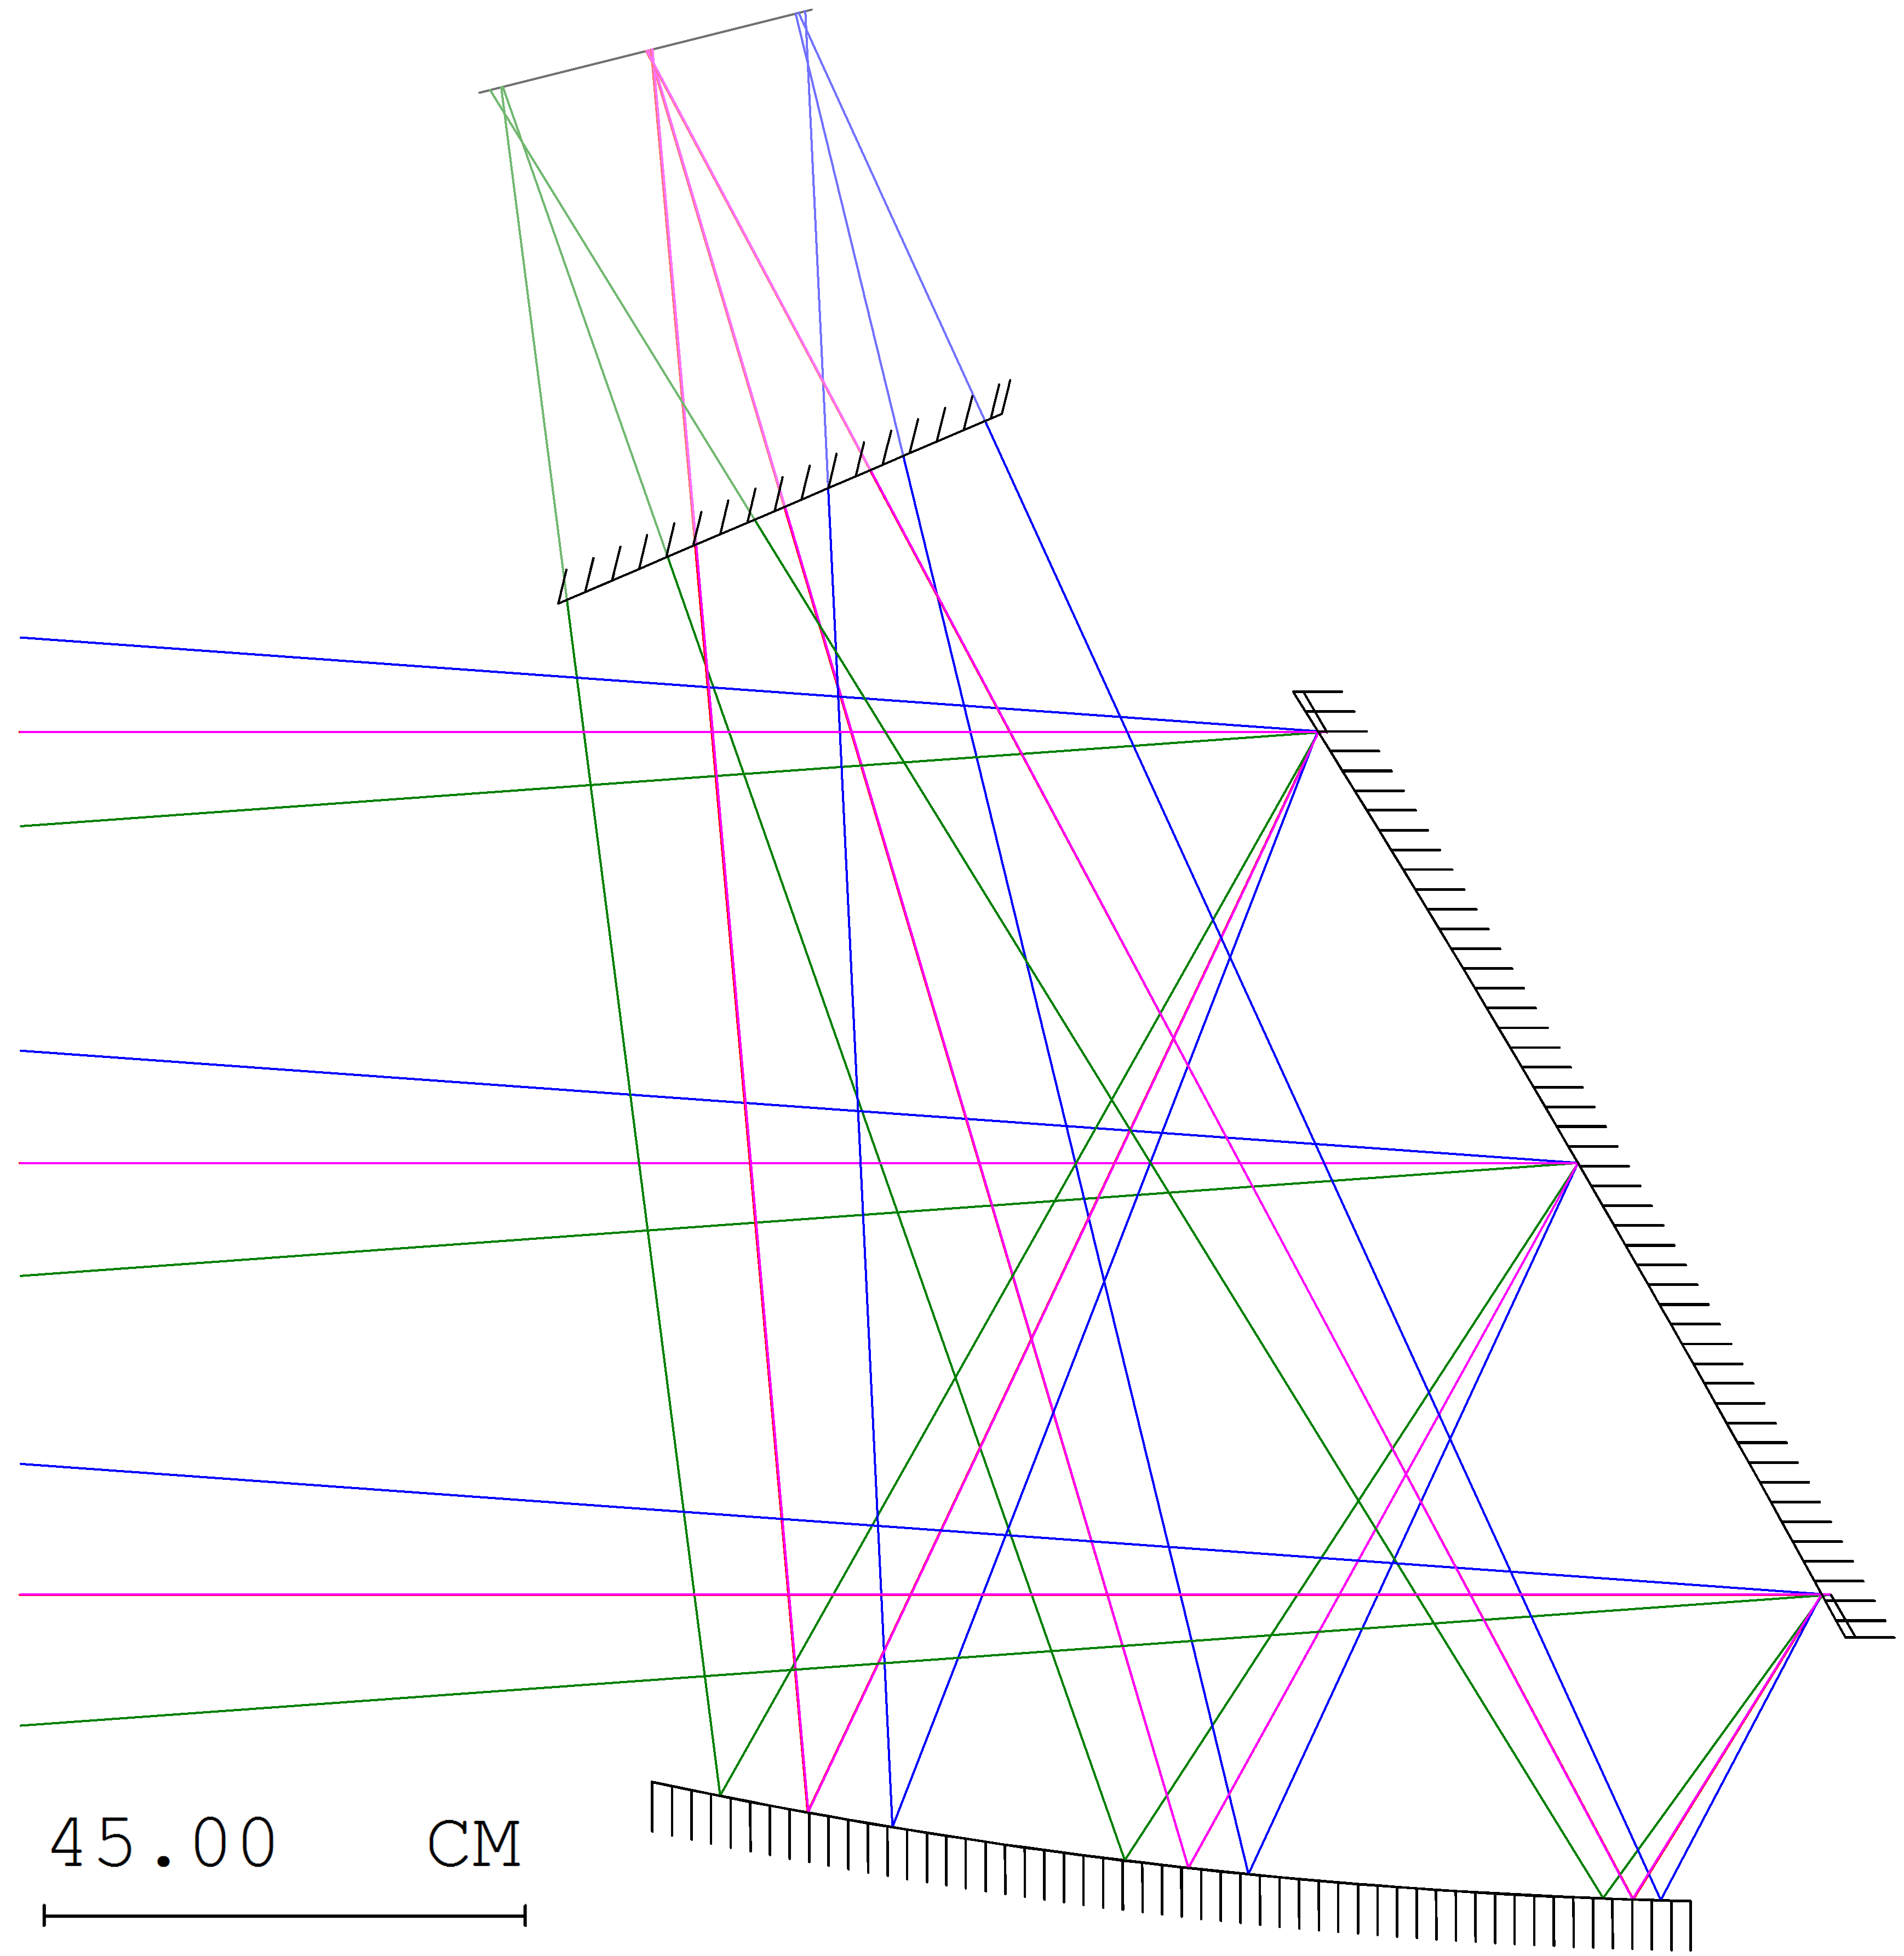
\includegraphics[width=10cm]{xdragone_raytrace.png} 
	\caption{Ray trace of the \coreplus design. Fields are at +4.1, 0, and -4.1 degrees. Rays are shown extending beyond the tertiary 
		to clearly show the focal plane.  In reality the tertiary folds these rays out of the page and toward the entrance 
		aperture.  
	}
	\label{fig:raytrace_xdragone}
\end{figure}

%strehl contours.  
\begin{figure}[htbp] %  figure placement: here, top, bottom, or page
	\centering
	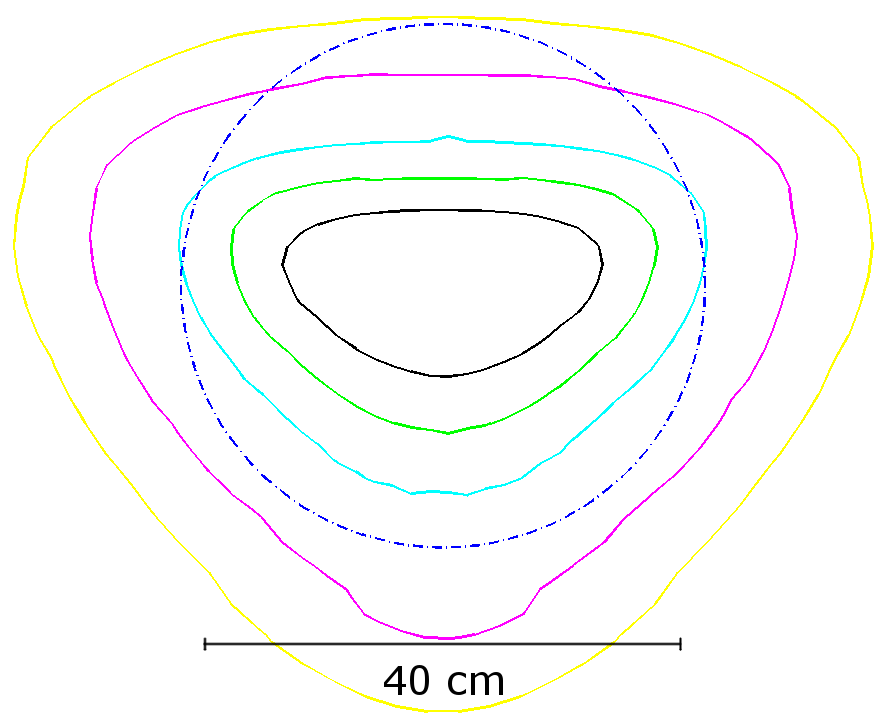
\includegraphics[width=12cm]{core_xdragone_strehl.png} 
	\caption{Strehl$=0.8$ contours defining the diffraction limited field of view of \coreplus at 
                 160~GHz (yellow), 220~GHz (magenta), 340~GHz (cyan), 450~GHz (green), and 600~GHz (black). 
		The usable field of view, limited by the ability to baffle the focal plane, is shown as a 
                dashed blue circle.
		}
	\label{fig:strehl_xdragone}
\end{figure}

With only two mirrors the system is too long to fit within the satellite envelope, so we added a flat 
tertiary mirror to fold the light path and make the system more compact.  This flat mirror 
could be replaced by a reflective polarization modulator. 


\noindent \textbf{Advantages}
\begin{itemize}
	\item Large, flat, telecentric focal plane.
	\item All mirrors are placed near the main satellite body simplifying the mounting structure.
\end{itemize}

\noindent \textbf{Disadvantages}
\begin{itemize}
	\item Large telescope is difficult to fit within payload volume.
	\item Large heavy mirrors are required.
	\item Has direct views of the focal plane to the sky and strong sidelobes.
	\item No convenient place for baffling or for an aperture stop to control sidelobes.
\end{itemize}


The largest difficulty with this crossed dragone system is baffling the focal plane to reject stray light 
from the sky.  In Figure~\ref{fig:raytrace_xdragone} the gray dashed line shows there is a direct path 
for objects about 70 degrees off boresight to directly illuminate the focal plane.  The fold mirror moves 
the focal plane closer to the entrance aperture, making baffling more complicated.  We added a `bucket' 
baffle around the focal plane (at ?? K) and a collar (at ?? K) around the entrance aperture of the system.  Additionally, we 
limit the focal plane to 4.1 degrees in radius.  Between the baffles and smaller focal plane there is no 
direct view of the focal plane from the sky.  The final focal plane size is shown by the blue dashed line 
in Figure~\ref{fig:strehl_xdragone} and is constrained by the baffling requirement rather than by Strehl 
ratios, which is the limit for the Gregorian design.

%strehl contours.  
\begin{figure}[htbp] %  figure placement: here, top, bottom, or page
	\centering
	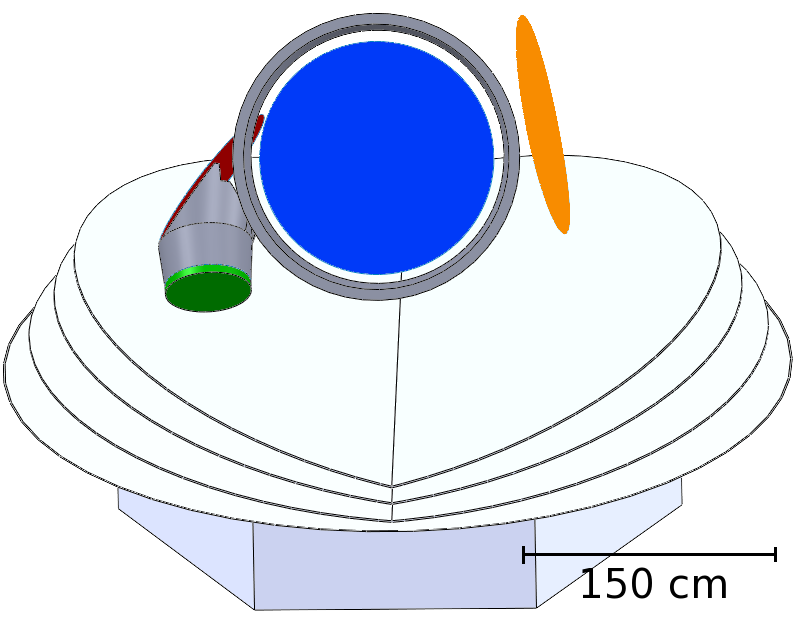
\includegraphics[width=10cm]{full_xdragone.png} 
	\caption{CAD model of the Crossed Dragone system.  The view is looking down the boresight of the telescope. The 
		primary is blue, the secondary orange, and the tertiary is red.  The focal plane is green and baffles are grey.
		Below the telescope the white sunshields and the satellite service module are shown.
		\comred{ky: This caption feels confusing to me. Suggestions? Also picture maybe isn't very clear. Suggestions there?}\comblue{Darragh: I think the caption reads fine. At first glance it is a bit difficult to figure out the positioning of the secondary relative to the primary - would a different projection clear that up?}
	}
	\label{fig:full_xdragone}
\end{figure}

The final optical system with tertiary mirrors and baffles is shown in Figure~\ref{fig:full_xdragone} and fits within 
the satellite envelope if 
$\alpha = 30$ and $\beta = 65$ \comred{will these have been defined somewhere else? or do we need to define them here}\comblue{Darragh: Based on the template, I think we may need to define them here}. 
Additionally the system is rotated about the bore-sight to lay roughly 
on its side.  This puts the mirrors and focal plane close to the main satellite body, reducing the need for 
heavy supports, and is the only orientation where the telescope fits within the baseline sun-shields. 

%an image to show the full system?  visualizing this is difficult.

%table of mirror sizes. other parameters??

\begin{table}[h!]
	\centering
	\begin{tabular}{|l|c|}
		%\hline
		%\multicolumn{2}{|c|}{\bf{Gregorian}} \\
		\hline
		Primary mirror   & 131~cm $\times$ 152~cm   \\
		Secondary mirror   & 125 cm $\times$ 146~cm  \\
		Tertiary mirror  & 104 cm $\times$ 74~cm    \\
		Focal ratio (F/\#)               & 2.54   \\
		\multicolumn{1}{|l|}{FOV, Focal plane diameter at Strehl $= 0.8$} & \\
		\multicolumn{1}{|c|}{@ 150 GHz}    & 4.1 deg $\times$ 4.1 deg, 87 F$\lambda \times 87 \text{~F}\lambda$ \\
		\hline
		
	\end{tabular}
	\caption{Parameters for the \coreplus Crossed Dragone design.  Mirror dimensions are the largest physical sizes.  Focal 
		plane dimensions are given at 150~GHz in degrees and in units of F$\lambda$ ($\lambda=2$~mm) to faciliate comparison between 
		designs with different F/\#'s.
		\comblue{Darragh: I will produce a similar table for the system with alumina lens (don't think it is necessary for the system without the lens, as that is an intermediate step in the Gregorian design process?)} }
	\label{tab:mirrors}
	
\end{table}

The major advantage of this system is a large, flat, telecentric focal plane which greatly simplifies 
the required detector architecture.  The main disadvantages are the three large, and therefore heavy, 
mirrors and the stringent baffling requirements which limit the usable focal plane area.  The benefit of 
a flat focal plane is sufficient that the Crossed Dragone is the current baseline for \coreplus. \comred{true?}

Sidelobes 
%(e.g. the 3 reflection crossed dragone sidelobe) 
other than direct views of the focal plane from 
the sky are currently being studied.

%====================================================================================

%====================================================================================
\bibliographystyle{aa}

%\small
%\bibliography{bibliography}
\clearpage
%\newpage
\newpage
\begin{thebibliography}{99}
	%
	%\bibitem{martin}
	%Mart\'in, E. L., Rebolo, R., \& Zapatero Osorio, M. R.
	%``Giant Exoplanets, Brown Dwarfs and Very Low Mass Stars,"
	%1996, ApJ, 469, 706
	%
	%\input bib_mapping_inflation.tex
	
	\bibitem{granet_2002} Granet C., Designing classical offset Cassegrain or Gregorian dual-reflector antennas from combinations of prescribed geometric parameters, 
	in IEEE Antennas and Propagation Magazine, vol. 44, no. 3, pp. 114-123, Jun 2002.
	doi: 10.1109/MAP.2002.1028736,
	URL: http://ieeexplore.ieee.org/stamp/stamp.jsp?arnumber=1028736

	\bibitem{tran_2008} Tran H., et al., Comparison of the crossed and the Gregorian Mizuguchi–Dragone for wide-field millimeter-wave astronomy, Applied Optics Vol. 47, Issue 2, pp. 103-109 (2008)  doi: 10.1364/AO.47.000103
	
	\bibitem{granet_2001} Granet C., Designing classical Dragonian offset dual-reflector antennas from combinations of prescribed geometric parameters, 
	in IEEE Antennas and Propagation Magazine, vol. 43, no. 6, pp. 100-107, Dec 2001.
	doi: 10.1109/74.979502,
	URL: http://ieeexplore.ieee.org/stamp/stamp.jsp?tp=\&arnumber=979502\&isnumber=21102
	
%	\bibitem{PRSM13} PRISM collaboration, PRISM, arXiv:1306.2259.
	
%	\bibitem{Bock09} Bock J., et al., astro.ph/0906.1188
	
%	\bibitem{Kogu11} A. Kogut et al., PIXIE, arXiv:1105.2044.
	
%	\bibitem{Hazu12} M. Hazumi et al. LiteBIRD, SPIE 2012.
	
%	\bibitem{Kend12} Kendrick Smith et al, JCAP, Issue 06, id. 014	 (2012)	
	
	
\end{thebibliography}

\end{document}